\subsubsection{}
\label{sec:analysis:research:analogs:imessage}

\textit{iMessage} -- проприетарное программное обеспечение от компании Apple, которое поставялется с дистрибьютивами почти всего семества современных операционных систем Apple:
\begin{itemize}
	\item iOS;
	\item macOS;
	\item watchOS.
\end{itemize}

iMessage интегрирован в приложения Messages на iOS и macOS, идентификаторами пользователей являются их мобильные номера или почта, привязанные к Apple ID. На рисунке \ref{sec:analysis:research:analogs:imessage:design} продемонстрирован дизайн приложения. Приложение поддерживает групповые чаты, расширения, является бесплатным для всех(и доступно только для) пользователей ОС, перечисленных выше.

\begin{figure}[h]
  \centering
    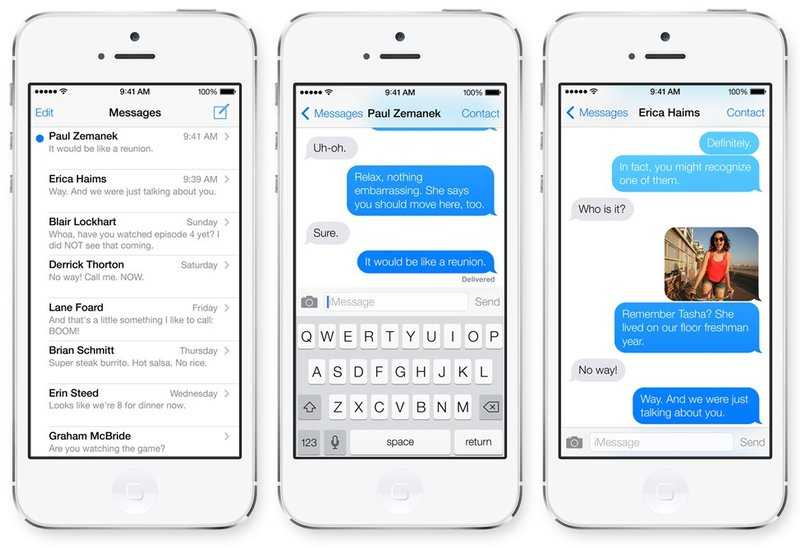
\includegraphics[width=0.75\textwidth]{inc/img/imdesign.jpeg}
  \caption{Дизайн iMessage}
  \label{sec:analysis:research:analogs:imessage:design}
\end{figure}

Коммуникационный протокол iMessage основан на Apple Push Notification Service -- прориетарном бинарном протоколе Apple. Телефон поддерживает постоянное соединение с серверами Apple, каждое соединение имеет собственный уникальный код, выступающий идентификатором. Соединение зашифровано при помощи TLS, используя сертификат устройства, который создаётся и отправляется на сервера Apple при активации утройства.
Криптографический протокол iMessage работает следующим образом:

\begin{enumerate}
	\item При активации iMessage на устройстве, генерируется две пары ассиметричных ключей: одна для шифрования и вторая для верификации.
	\item Публичные ключи отправляются на сервера Apple, а приватные никогда не покидают устройство.
	\item Когда кто-то начинает диалог, его устройство получает все публичные ключи участвников диалога.
	\item При отправке сообщения, формируется \(n\) сообщений, каждое зашифрованно \(i\)-ым публичным ключом, где \(n\) -- количество устройств в диалоге.
\end{enumerate}

Недостатком данного подхода является потенциальная возможность Apple добавить собственный публичный ключ в список публичных ключей получателя, таким образом получив свою копию зашифрованного сообщения.